\section{Auswertung und Visualisierung der Daten}
Für die Auswertung der Daten und die daraus resultierenden Visualisierung muss zunächst definiert werden, welche Kriterien für das Dashboard relevant sind. Im Folgenden wird genauer darauf eingegangen, wie die \textit{wichtigen} Werte aus den bereitstehenden Daten ermittelt werden und welche Methode genutzt werden soll, um diese zu visualisieren.

\subsection{Auswertung}
Ein Dashboard ist eine Darstellungsoption, mit der es einem Benutzer gelingen soll, einen Gesamtüberblick über die für ihn wichtigen Daten zu erhalten. Um diesen Gesamtüberblick erstellen zu können, muss eine Analyse des Benutzers vorgenommen werden, um zu ermitteln, welche Daten für ihn von Bedeutung sind. \cite{few_2013}

Da vorab festgelegt wurde, dass die Webapplikation ohne Benutzerregistrierung auskommen soll, können die Daten nicht direkt auf den Benutzer zugeschnitten werden, der seine Spielergebnisse hochlädt. Die Herausforderung besteht nun darin, Werte zu ermitteln, die für den Benutzer von Bedeutung sind, ohne einen persönlichen Bezug herstellen zu können. Dieser Aspekt resultiert darin, dass das Dashboard von mehreren Benutzergruppen genutzt wird. Es muss dementsprechend so konzeptioniert werden, dass Benutzer, die ihre Spielergebnisse hochladen, ihre wichtigen Daten erhalten, aber auch dass die Benutzer wichtige Informationen erhalten, die ihre Spielergebnisse nicht hochladen, wichtige Informationen erhalten. Die daraus resultierenden, für wichtig erachteten Werte, werden im Folgenden aufgelistet und diskutiert.

\subsubsection{Total Sheets}
Der erste Wert, der für relevant erachtet wird, ist die Summe der hochgeladenen handgeschriebenen Zettel. Da bei einem Kniffelspiel nicht immer alle sechs Spiele auf einem Zettel gespielt werden, kann dieser Wert die Anzahl der gespielten Sitzungen darlegen. Dieser Wert bietet darüber hinaus einen Indikator für die Nutzung der Webapplikation, da dieser Wert gleich ist mit der Anzahl der erfolgreichen Nutzung der Hochladen-Funktion. Mit dieser Angabe können die Nutzer einen Überblick über die gespielten Sitzungen erhalten und die Entwickler einen Überblick über die Nutzung der App.

\subsubsection{First Upload}
Der zweite Wert ist der Zeitpunkt, an dem der erste erfolgreiche Upload stattgefunden hat. Dieser Wert gibt Auskunft darüber, wie lange die App in Benutzung ist und wie sich die Daten über den Zeitraum entwickeln. Der Nutzer soll also mit der Angabe einen zeitlichen Überblick über die Berechnung der Daten erhalten, um diese besser einzuschätzen. Der Wert wird als ein Datum mit Tag, Monat und Jahr angegeben.

\subsubsection{Total Yahtzees}
Dieser Wert gibt Auskunft über die Summe der \textit{Yahtzees}, die über alle Spiele hinweg gewürfelt wurden. Ein \textit{Yahtzee}, oder auch \textit{Kniffel} genannt wird gewürfelt, wenn alle Würfel die gleiche Augenzahl haben. Es ist das höchste Ergebnis, das ein Spieler mit einem Wurf erreichen kann. Dieser Wert ist daher von großer Wichtigkeit für einen Spieler. Im Zusammenhang mit dem ersten Wert kann der Nutzer einen Überblick über die Relation der Kniffel und der gespielten Sitzungen erhalten.

\subsubsection{Total Score}
Der vierte Wert gibt die Summe der erreichten Punkte für alle Spiele an. Dieser Wert hat keine besondere statistische Bedeutung, es soll lediglich als ein Wert dargestellt werden, der die Nutzer begeistert.

\subsubsection{Highest Score}
Der \textit{Highest Score}-Wert soll die höchste erreichte Punktzahl eines Spielers, die mit einem Blatt erreicht wurde, darstellen. Da es verschiedenen Spielweisen des Spiels gibt, kann dieser Wert mehr aussagen, als wenn der höchste Wert eines Spiels eines Blattes genommen werden würde. Ein Nutzer kann somit einen Überblick über die Höchstpunktzahl erhalten, die ein Spieler erreicht hat.

\subsubsection{Average Score}
Der letzte Wert soll die durchschnittliche Punktzahl angeben, die in einer Sitzung erreicht wurde. Ähnlich wie beim \textit{Highest Score}-Wert, wird dieser Wert nicht auf Basis der einzelnen Spiele auf einem Blatt ermittelt, sondern auf Basis der gesamten Sitzung. Es wird also das arithmetische Mittel über die Anzahl der \textit{Total Sheets} und die Anzahl \textit{Total Score} errechnet.

\subsection{Visualisierung} \label{sec:visualisation}
Bei der Visualisierung kommt es darauf an, dass die Gesamtheit der Daten so präsentiert wird, dass diese einfach und zugänglich sind. Das schließt zum einen die optische Darstellung ein, aber auch die Navigation und Interaktion mit den Daten. Hierbei ist wiederum zu beachten, zu welcher Benutzergruppe eine Person gehört, da sich daraus die womögliche Medienkompetenz eines Nutzers ableiten lässt. \cite{few_2013}
Das Ziel vom Dashboard soll es sein, die Daten möglichst zugänglich für jede Benutzergruppe zu machen. Aufgrund dessen sollen alle Daten, auf einem Blick erkennbar sein, sodass keine umfangreiche Navigation erforderlich ist, wie zum Beispiel eine Scroll-Bewegung.
Die Abbildung \ref{fig:mockup} soll ein \textit{MockUp} darstellen, wie die Darstellung der als wichtig definierten Werte aussehen könnte.
Zusätzlich zu der einfachen Darstellung der Daten werden die Daten auch in einer grafischen Darstellung dargestellt. In dem Graphen sollen die Daten in Zusammenhang mit der Zeit dargestellt werden, um so Trends in den hochgeladenen Spielen genauer erkennen zu können.

\begin{figure}[H]
	\centering
	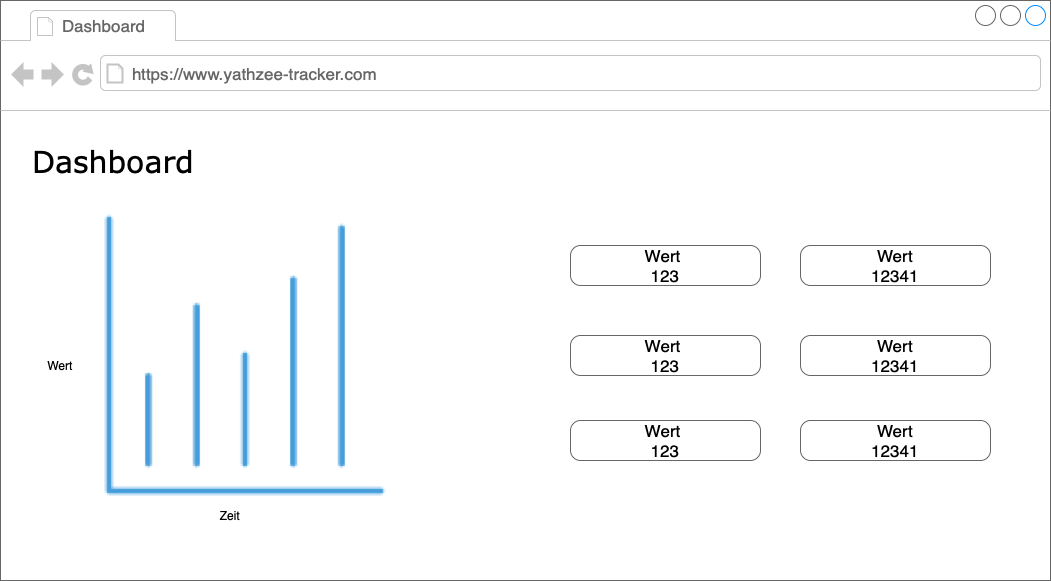
\includegraphics[width=\imgMed]{images/practice/dashboard_mockup.png}
	\caption{MockUp für die Visualisierung der Daten}
	\label{fig:mockup}
\end{figure}
